\chapter{Research Methodology and Data}

This chapter focuses on describing which approaches were chosen for the task at hand and why, as well as shows how the work progressed. 

\section{Core Concepts}

To reiterate the current problem is to find out if \gls{gnn} can compete at solving the \gls{mwm} problem compared to other approximation methods such as greedy algorithm.

Before properly describing the choices made for approaching this problem, it is worth going through basic concepts of \gls{gnn}s and neural networks in general. It is common to think of neural networks as of a black box where you give some data to this box and it tries to predict the correct answer. In this case the data is a graph consisting of vertices connected by edges that have weights and the expected answer should be pairs of vertices that were matched together.



\section{Challenges}

As mentioned the idea behind supervised learning is to give a model the correct answers so it can by trial and error learn from it. Theese answers are not included the initial datasets so the optimal solutions need to be calculated. Blossom algorithm implemented by Joris van Rantwijk in Python was used \cite{mwmBlossom}. This does however point out an important weakness of the supervised approach. Obviously a model needs to be able to handle graphs of different sizes and it is the large ones that are most interesting. Finding an optimal \gls{mwm} for the large graphs can be time consuming, at the same time a model need as much data as possible to learn leading to multiple large graphs consuming to much time. This poses a question whether it is possible for the model to learn on small and medium sized graphs that are not as time consuming and transfer learned patterns to solve larger graphs.

Another important aspect that must be taken in to the consideration is that it is unlikely for the model to fully follow the restuctions of the problem. Model might decide to match same node to 2 neighbors at the same time, which should not be allowed. 

\section{Main Idea}

To summarize, given a weighted udirected graph, the \gls{nn} must predict  a valid subset of edges or in other words pairs of vertices that maximizes the total weight. The \gls{nn} will have a graph as an input and the otput will be the probabilities (0.00 - 1.00) of how likely an edge will be in the matching. To control that a solution is valid, instead of picking all the edges with the probability higher than 50\%, the edges can be sorted by their probabilities and greedily picked in that order if they don't break the validity of the solution. This might sound illogical to use greedy algorithm on the models output to beat the normal greedy algorithm with weights, but the fact that edges are now sorted not by their weight, but a score decided by \gls{nn} does make a difference, since the \gls{gnn} can take multiple features in consideration when assigning probabilities. Some of theese features come naturaly such as structure of the graph, and some we can manualy add during preprocessing. 

\gls{nn}s have a lot of hyperparameters and other methods that can be tuned to make a model better suited for the task. The ideal way of finding the best combination of the hyperparameters is to try as many combinations as possible and train a model for each combination, and choose the one with best performance. This is a time consuming procedure however and therefore in this task the exploration of hyperparameters was narrowed down. 

During the experiments following hyperparameters were tested:

Hyperparameters:

1. Learning rate
2. Class weights
3. Weight decay
4. Network depth and width (layers and neurons)

Additionally other methods were tried such as:

1. Augmenting data (adding extra features to the nodes during preproccessing)
	1.1 degree, weights relative to the neighbors, difference between weights of the neighbors, sums of the weights. Also for the edge classification 1st largest weight, 2nd largest weight were added to match the reduction rule that was tested later.

Steps:

Trying line graph First

100 graphs from MNIST

1. Staring with the most default type of the nework with 2 layers and 64 neurons each
	Network gets to heavily influenced by class disbalance. There are more edges that are supposed to be dropped compared to those that must be in the matching.
2. Adding classweight
3. Adjusting learning rate. To high learing rates resulted in too instable loss function, too low learning rate did not give enough progress and was too slow. Value of 0.001 worked well as middle ground
4. Augmenting node features. Trying each additional feature one by one to see it they have any benefits by themselves and then adding them all together since they can mostly be calculated simultaneously.

Result are getting closer to beating greedy, but converting to the line graph was consuming to much time. Trying edge classification. With same hyperparameters and repurposed node feature augmentation.

1. Edge classification is a little bit worse on average. In theory it can be due to line graph containing more structural information in it compared to original.
2. Trying to add a reduction rule and 2 additional features:  1st largest weight, 2nd largest weight for each node.
3. Improvements seemed to stagnate.

Trying to train graph on the whole dataset of 55000 graphs:









\section{Data}

The model should be capable of solving any graph relevant to \gls{mwm} problem. A relevant graph can be difined by following characterisitcs
Ideally the model should be able to handle any kind of an udirected graph with weighted edges.

For training and experimenting with the \gls{gnn}, a MNIST dataset was used \cite{dwivedi2022benchmarking}. The dataset consists of 70000 relatively small graphs with 70 nodes and 564 edges on average. Graphs also include features for the edges representing distances between node. Theese features is what is used as the weights for the problem. Although the graphs in this dataset are realatively small they have some fitting qualities such and nodes having many neighbors creating more possible ways to match the nodes. Small size also makes it less time consuming to train the models and try different approaches as well as shows whether a \gls{gnn} trained on smaller graphs can transfer its knowledge to larger graphs.

A couple large graphs from SuiteSparse were chosen for testing performance on large graphs.

Small handcrafted graphs were used to test if \gls{gnn} can at least beat the cases specificaly made to abuse weaknesses of a greedy approach.

\section{Expected Results}

\subsection{Accuracy and total weight}

There are not that many researches specifically for \gls{mwm}, but problems like \gls{mis} that are relatively close to \gls{mwm} can indicate similar results for this case as well. As discussed in the \hyperref[sec:background]{Background section}, there are researches that show that \gls{gnn}s are capable of solving \gls{co} problems and beating greedy algorithms, while other rather indicate that improvements are still needed for it to be worth using. Therefore it is hard to forecast any results based on previous work. Nothing stands in the way of being optimistic however, additionally to the fact that greedy algorithm is relatively simple and \gls{nn} should be able the recognise a more complex pattern it can use to achieve better results. It is absolutely not expected for the model to be able to find optimal solution since any \gls{nn} is a heuristic. The margin by which \gls{gnn} can surpass the greedy solution is expected to be rather small, since from the data analysis it was abserved that for the majority of graphs greedy algorithm preforms rather well with above 80\% of the optimal possible weight.

\subsection{Time}

\gls{gnn} model is a heuristic solver and gives an approximate answer. Therefore model should be noticeably faster than exact algorithm, otherwise it would not be worth it. The time a model takes to solve one instance of a problem should be closer to that of a greedy algorithm and probably slightly longer due to preproccessing required such as augmenting data with adittional features. Naturaly, time will also depend on the depth and the width of the network.

\section{Model Architecture}

\section{Line Graph Approach}

Line graph approach was the first attempt at using a simple \gls{gnn}, which later turned out to be too time consuming for larger graphs to be worth further expriements. It did however give some usefull insight as well as a showed to be a proof of concept. In the context of graphs line graph is a complement of the original graph that turns each edge to a vertex and connects the vertices is they shared a vertex in the original graph. 

Nouranizadeh et. al. showed anothing approach at solving \gls{mis} \cite{DBLPjournals/corr/abs-2107-01410}.

Examaple of a graph and its line graph convertion
\begin{figure}[H]
    \centering
    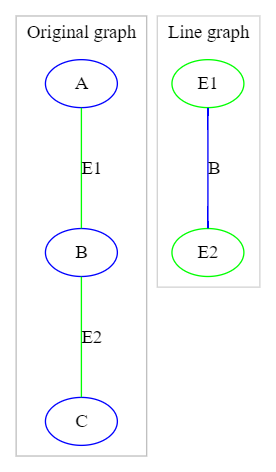
\includegraphics[scale=0.5]{figures/LineGraphExample}
    \caption{Original graph (left) and its line graph (right)}
    \label{Line graph figure}
\end{figure}

\subsection{Progress}

1. bare bones
2. class weights -> all or nothing
3. optimizer learning rate, network depth and width, 
4. skip connections
5. extra features

\section{Edge Classification Approach}

A more natural way of approaching this problem is for each pair of vertices that are conneced by an edge, ask the model if given pair should be a part of the matching. In other words model is classifying an edge. 

\subsection{Progress}

\section{Result Validation}

\begin{enumerate}
\item Time - how long an algorithm took to produce an answer.
\item Correctness - is the answer correct. In case of \gls{mwm} the total weight aquired would be the measurement of how correct the solution is. It is unlikely that \gls{gnn} can find an optimal solution for more complex problems so it is reasonable to look at how close \gls{gnn} comes to the optimal solution.
\item Memory - how much memory is needed. However in this project there is less of a focus on memory
\end{enumerate}

All the experiments have been done on the same machine with: 11th Gen Intel(R) Core(TM) i7-11700K 3.60GHz 8-core CPU, 16 GB RAM and NVIDIA RTX 3080Ti graphics card.


